\section{Validation (Preliminary results)}
\label{sec:validation}

All preliminary computations presented below have good to excellent agreement with experimental data. Details of each of the cases, like the number of cells used, computation time, and Tera-flops achieved will be included in the final paper.

The figure labels below may contain symbols and variables not explained in this working version of the paper.

\subsection{Flat Plate}
Computations of the flow over a flat plate have been performed and validated against the results from the high-order workshop. We obtained a $C_{d}$ value of 1.3112e-3 matching with results from the workshop. A detailed description of convergence and error vs. work-units will be presented in the final draft.  

\subsection{Circular Cylinder}
\begin{figure}
\centering
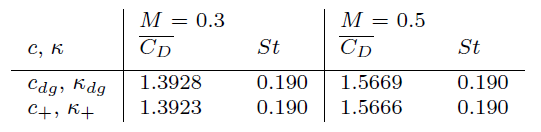
\includegraphics[height=20mm]{./figures/table_925} \\
\caption{Values of the time-averaged drag coefficient and Strouhal number for the circular cylinder in flows with $M = 0.3$ and $M = 0.5$. The flows were simulated using the VCJH schemes with $p = 2, c = c_{dg}, \kappa = \kappa_{dg} and c = c_+, \kappa = \kappa_+$ in conjunction with the Rusanov flux with $\lambda = 1$ and the LDG flux with $\beta = ±0.5n$ and $\tau = 0.1$ on the unstructured triangular grid with $N = 63472$ elements.}
\label{fig:table_925}
\end{figure}

\begin{figure}
\centering
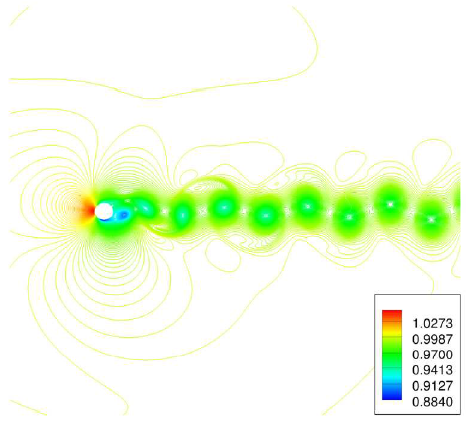
\includegraphics[height=60mm]{./figures/figure_921a} \\
\caption{Density contour for the flow with $M = 0.3$ around the circular cylinder.}
\label{fig:figure_921a}
\end{figure}

\begin{figure}
\centering
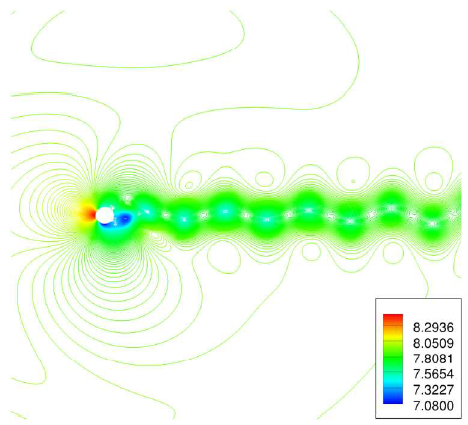
\includegraphics[height=60mm]{./figures/figure_921b} \\
\caption{Pressure contour for the flow with $M = 0.3$ around the circular cylinder.}
\label{fig:figure_921b}
\end{figure}

\begin{figure}
\centering
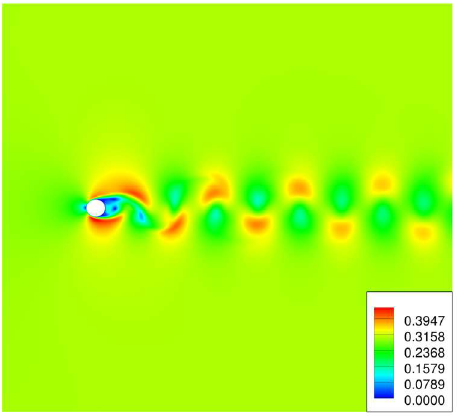
\includegraphics[height=60mm]{./figures/figure_922a} \\
\caption{Mach contour for the flow with $M = 0.3$ around the circular cylinder.}
\label{fig:figure_922a}
\end{figure}

\begin{figure}
\centering
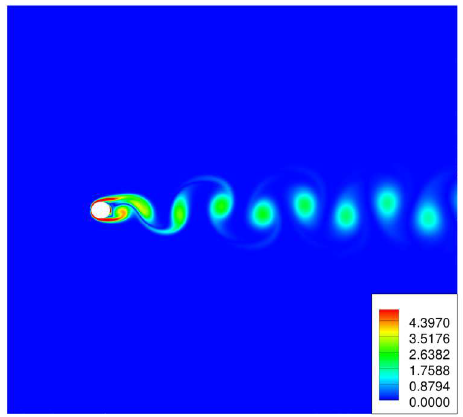
\includegraphics[height=60mm]{./figures/figure_922b} \\
\caption{Vorticity contour for the flow with $M = 0.3$ around the circular cylinder.}
\label{fig:figure_922b}
\end{figure}

\begin{figure}
\centering
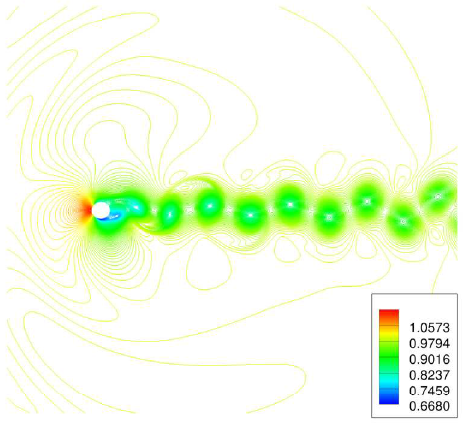
\includegraphics[height=60mm]{./figures/figure_923a} \\
\caption{Density contour for the flow with $M = 0.5$ around the circular cylinder.}
\label{fig:figure_923a}
\end{figure}

\begin{figure}
\centering
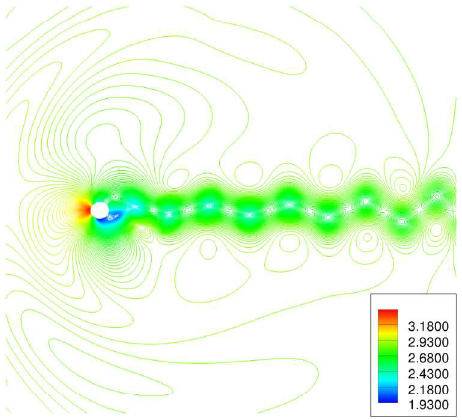
\includegraphics[height=60mm]{./figures/figure_923b} \\
\caption{Pressure contour for the flow with $M = 0.5$ around the circular cylinder.}
\label{fig:figure_923b}
\end{figure}

\begin{figure}
\centering
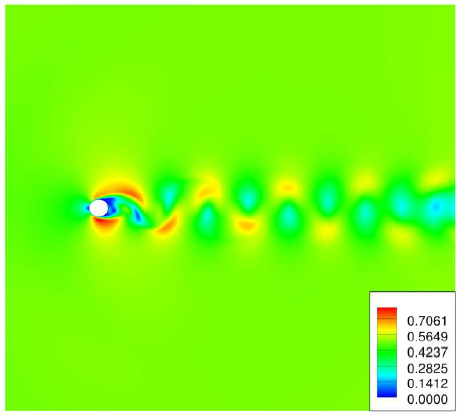
\includegraphics[height=60mm]{./figures/figure_924a} \\
\caption{Mach contour for the flow with $M = 0.5$ around the circular cylinder.}
\label{fig:figure_924a}
\end{figure}

\begin{figure}
\centering
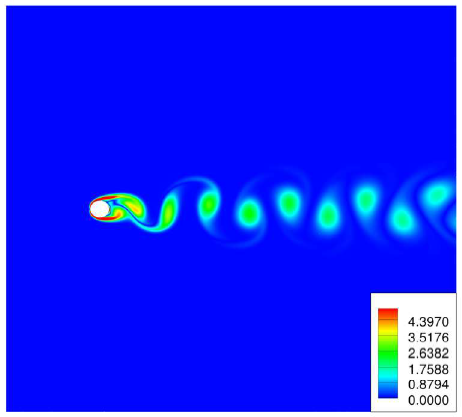
\includegraphics[height=60mm]{./figures/figure_924b} \\
\caption{Vorticity contour for the flow with $M = 0.5$ around the circular cylinder.}
\label{fig:figure_924b}
\end{figure}
\newpage
%\subsubsection{Vortex transport by uniform flow (2D)}
%\subsubsection{Transonic Ringleb Flow (2D)}
%\subsubsection{Flow over an Analytical Body of Revolution (3D)}
\subsection{SD7003 airfoil at 4$\degr$ angle of attack}
From Williams's thesis\cite{williams2013thesis}

\begin{figure}
\centering
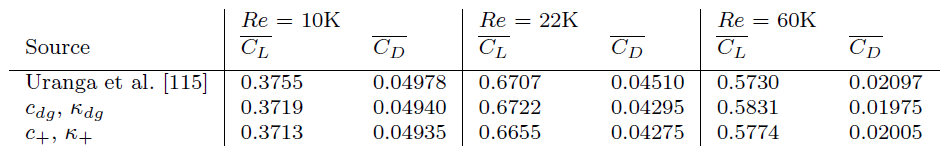
\includegraphics[height=30mm]{./figures/table_926} \\
\caption{Time-averaged values of the lift and drag coefficients for the SD7003 airfoil flows with $Re = 10000, 22000, 60000$}
\label{fig:table_926}
\end{figure}

\begin{figure}
\centering
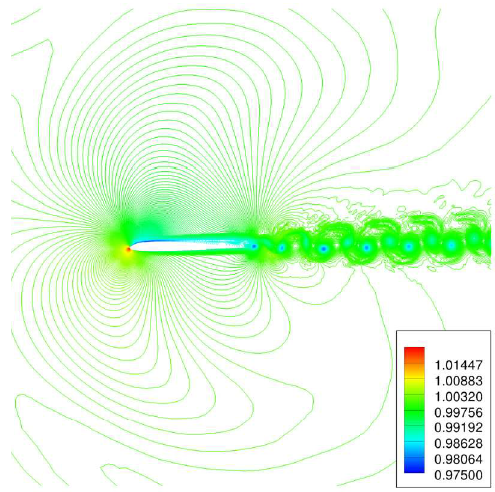
\includegraphics[height=60mm]{./figures/figure_935a} \\
\caption{Density contour for the flow with $Re = 10000$ around the SD7003 airfoil.}
\label{fig:figure_935a}
\end{figure}

\begin{figure}
\centering
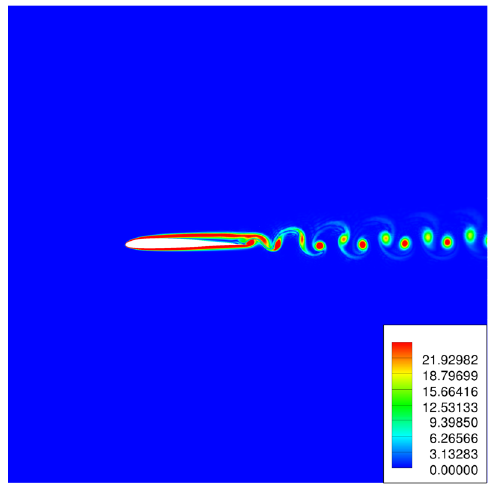
\includegraphics[height=60mm]{./figures/figure_935b} \\
\caption{Vorticity contour for the flow with $Re = 10000$ around the SD7003 airfoil.}
\label{fig:figure_935b}
\end{figure}

\begin{figure}
\centering
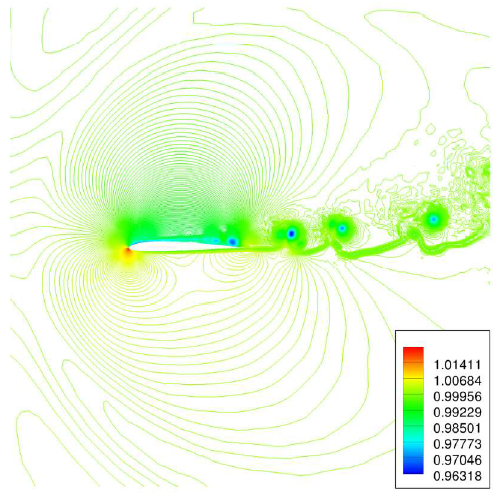
\includegraphics[height=60mm]{./figures/figure_936a} \\
\caption{Density contour for the flow with $Re = 22000$ around the SD7003 airfoil.}
\label{fig:figure_936a}
\end{figure}

\begin{figure}
\centering
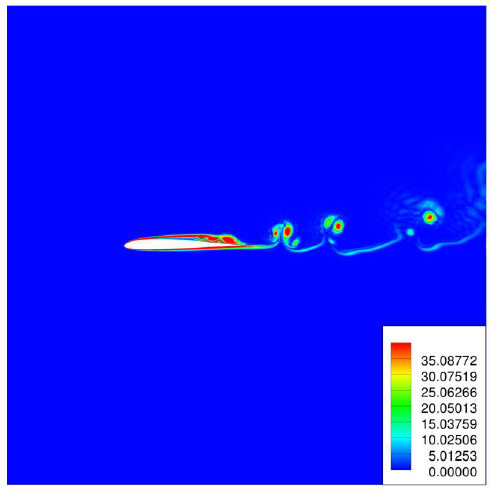
\includegraphics[height=60mm]{./figures/figure_936b} \\
\caption{Vorticity contour for the flow with $Re = 22000$ around the SD7003 airfoil.}
\label{fig:figure_936b}
\end{figure}

\begin{figure}
\centering
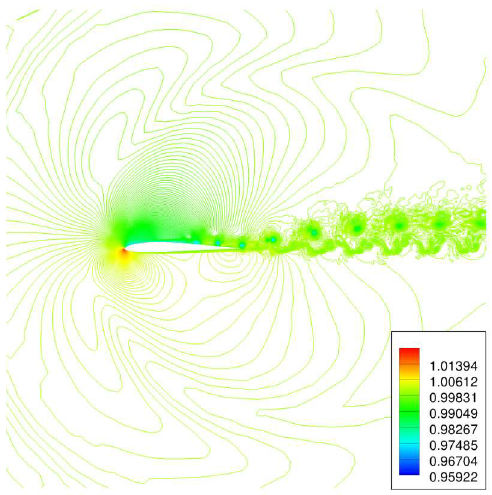
\includegraphics[height=60mm]{./figures/figure_937a} \\
\caption{Density contour for the flow with $Re = 60000$ around the SD7003 airfoil.}
\label{fig:figure_937a}
\end{figure}

\begin{figure}
\centering
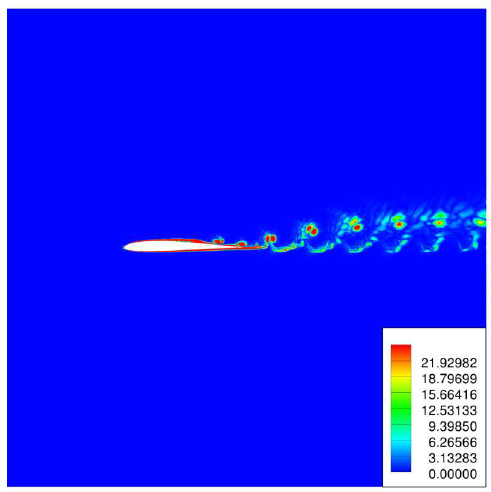
\includegraphics[height=60mm]{./figures/figure_937b} \\
\caption{Vorticity contour for the flow with $Re = 60000$ around the SD7003 airfoil.}
\label{fig:figure_937b}
\end{figure}
\newpage
\subsection{SD7003 wing section at 4$\degr$ angle of attack}
From David's thesis.
%\subsubsection{Laminar Flow around a Delta Wing}

\begin{figure}
\centering
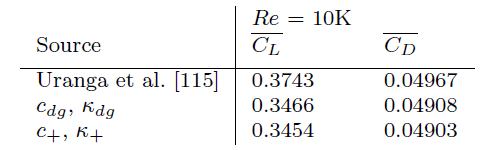
\includegraphics[height=20mm]{./figures/table_927} \\
\caption{Time-averaged values of the lift and drag coefficients for the SD7003 wing-section in a flow with $Re = 10000$}
\label{fig:table_927}
\end{figure}

\begin{figure}
\centering
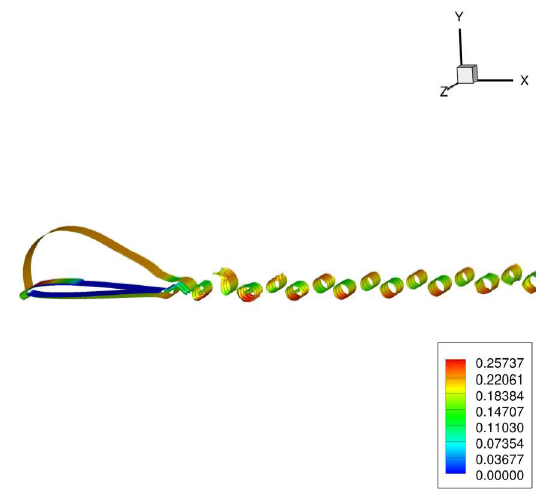
\includegraphics[height=60mm]{./figures/figure_939a} \\
\caption{Density isosurfaces colored by Mach number for the flow with $Re = 10000$ around the SD7003 wing-section.}
\label{fig:figure_939a}
\end{figure}

\begin{figure}
\centering
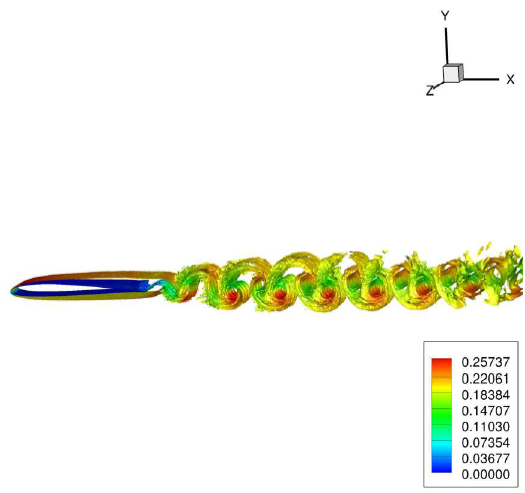
\includegraphics[height=60mm]{./figures/figure_939b} \\
\caption{Vorticity isosurfaces colored by Mach number for the flow with $Re = 10000$ around the SD7003 wing-section.}
\label{fig:figure_939b}
\end{figure}
\newpage
\subsection{DNS/LES of the Taylor-Green Vortex at Re = 1,600}
The results presented below were obtained using the recently-developed LES capabilities of HiFiLES. The fact that the grid with one eighth 
\begin{figure}
\centering
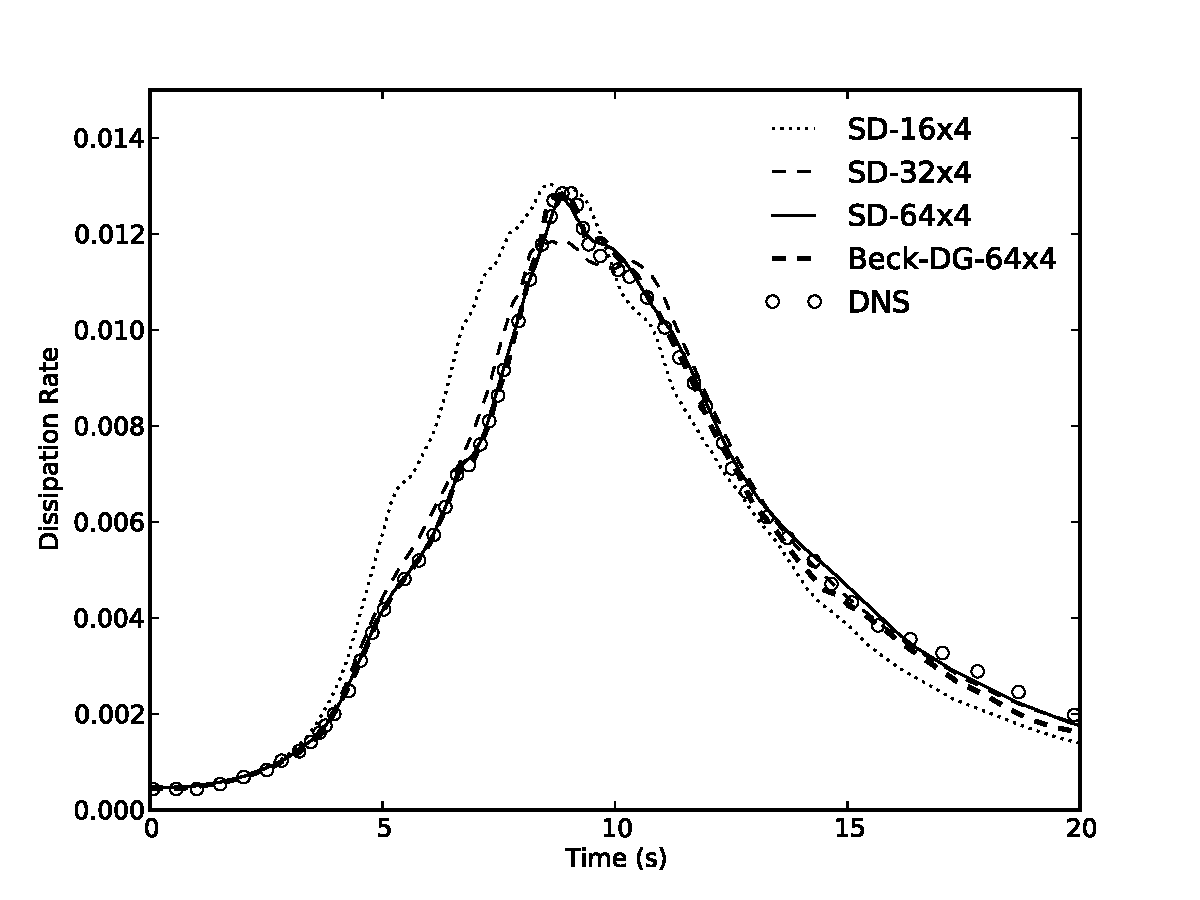
\includegraphics[height=60mm]{./figures/dissrate-hex-mesh-small.pdf} \\
\caption{LES of Tyalor-Green Vortex at Re=1,600\cite{bull2013a}}
\label{fig:setup}
\end{figure}

\newpage
\subsection{DNS of Decaying Homogeneous Turbulence}
Plots of turbulent kinetic energy and Reynolds stresses versus time will be presented.
\subsection{LES of Decaying Homogeneous Turbulence}
Plots of turbulent kinetic energy and Reynolds stresses versus time will be compared to the DNS results.


